\documentclass{sigchi}
\usepackage{subfigure, graphicx, url}

\newcommand{\strong}[1] {\textbf{#1}}
\newcommand{\code}[1] {\texttt{#1}}

\begin{document}
\title{Grammatical Relationships for non Linguists}
\numberofauthors{2}

\author{% 1st. author
\alignauthor First Lastname\\
% 2nd. author
\alignauthor {Firstname Lastname}\\
}

\maketitle

\begin{abstract}

\end{abstract}

\section{Introduction}

What does $X$ do? How is $Y$ described? Most analysts and researchers ask themselves these questions while trying to understand a subject.  So far, the field of information retrieval has tackled this problem indirectly: the analyst enters a search query, and the system returns some results. When the underlying data has structure, queries can be specific and targeted -- and there is now a substantial body of work [cite] on how best to issue structured queries over \emph{structured} data. But what if the ``data" is is text -- medical literature, legal records, interview transcripts? Although text is richly structured by rules of  grammar and narrative, it is rarely treated as such. While there is a lot of work on extracting various kinds of structured information from text, there is little on how to make it easy for users to access and query over it.  As the questions above show, however, structured queries over language can be extremely useful. In grammatical terms, they become ``What are the verbs of which $X$ is the subject?'' ``What are the adjectives that modify $Y$?''

Adapting existing structured-query interfaces to grammatical search is problematic for several reasons. The first is that the structures in language are not explicit, like columns in a table, but are implicit, and have to be extracted computationally. Only in the last decade have computational linguistic technologies become fast and accu rate enough to use in the real world.

The second problem is the lack of programming experience among searchers. Current structured query languages like SPARQL have complex syntaxes that require time and effort to learn. For example, here is a SPARQL query for ``What are all the country capitals in Africa?'':
\begin{verbatim}
SELECT ?capital ?country
WHERE {
  ?x cityname ?capital ;
     isCapitalOf ?y .
  ?y countryname ?country ;
     isInContinent Africa .
}
\end{verbatim}
Even if we assume that only professional analysts engaging in information-intensive work would want to issue such targeted queries,  programming experience is scarce. One study on a query language for selecting phrase structures from sentences found that that only 50\% of the people who wanted to use it had programming experience \cite{}.

The third problem is that there are no common-language terms for grammatical relationships even though ordinary people are perfectly capable of understanding and using them. Modern parsers use standard linguistics terminology to label their outputs, but those technical names and definitions are not always accessible to those outside the field. Take the phrases ``he threw the ball" and ``the ball was thrown by him". In both cases, it is clear that `he' is is the one who `threw' whereas, in grammatical terms, the first phrase is in the active case, and the phrase is in the passive case. The Stanford Dependency Parser \cite{}, for example, outputs two different variants of the verb-subject relation: \code{nsubj(he, threw)} and \code{nsubjpass(he, threw)}. A grammatical search system therefore has to bridge the gap between the relations that are recognizable to people and the relations that are extracted from the data

We conducted an experiment to investigate how grammatical relationships between words in English can be made more recognizable to ordinary people. Following the principle of recognition over recall, we hypothesized that examples would help people identify grammatical relationships more accurately rather than technical names.

Our results confirm that showing examples significantly improves the accuracy with which grammatical relationships are recognized. Participants identified grammatical relationships more accurately in all cases when they were  shown examples of words or phrases that matched.

Our findings also suggested that different types of relations benefited differently from words and phrases. In a follow-up experiment, we found that if distinctive or closed-class words tend to participate in a grammatical relationship, then a list of matching words is the best recognition aid. By contrast, in clausal or long-distance relationships, where the context determines how the two words are related, a list of phrases is best.

The rest of this paper is structured as follows. In the next section, we summarize the previous work on issuing structured queries over linguistic information extracted from text data. Then, we  describe our experiments and analyze the results. Finally, we summarize our findings and discuss their implications for grammatical search interfaces.

\section{Experiment 1: do Examples Help?}

\subsection{Hypothesis}
Our experiment's goal was to find out whether grammatical relationships could be made more recognizable by showing examples of their usage. We tested two types of examples: a list of matching words and a list of matching phrases containing the relationship. These alternatives correspond to the explicitly visible and implicitly-inferred portions of a grammatical relation. The words are explicitly visible in the text, but the grammatical relationship is implicitly inferred from contextual information such as the part of speech of the verb, the relative ordering, and any accompanying words.

Our hypothesis was the following:
\begin{quote}
	H1. Grammatical relations can be made more recognizable by showing examples of words or phrases that match.
\end{quote}


\begin{figure}
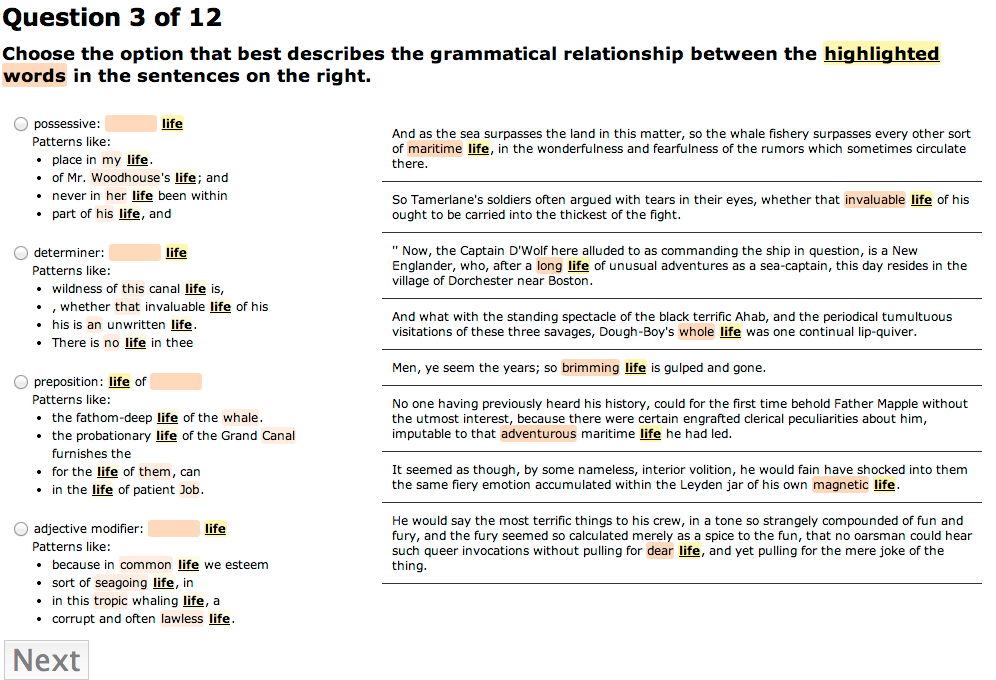
\includegraphics[width=\columnwidth]{fig/task}
\caption{\label{fig:task} An example of an identification task in the \emph{phrases} condition, for the relationship \code{amod(life, \_\_\_)}.}
\end{figure}

To test it, we presented participants with a series of identification tasks. In each task (Figure \ref{fig:task}), they were shown a list of sentences in which a particular grammatical relationship existed between two highlighted words. They were asked to identify which relationship it was from a list of four options.  Using a between-subjects design, we tested different strategies for presenting these options. Our goal was to see whether participants to whom we showed example usages identified the relationships more accurately than those to whom we did not.

\subsection{Variables}

\subsubsection{Presentation}

\begin{figure}
\subfigure[The baseline condition]{
	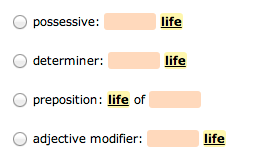
\includegraphics[width=0.5\columnwidth]{fig/baseline-choices}
    \label{fig:baseline-choices}
}
\subfigure[The matching-words condition]{
	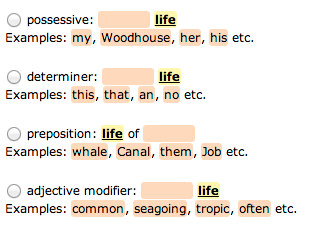
\includegraphics[width=0.3\columnwidth]{fig/words-choices}
    \label{fig:words-choices}
}
\caption{\label{fig:choices} The way the choices appeared in the three experiment conditions, for the relationship \code{amod(life, \_\_\_)} (where different adjectives modify the noun `life')}
\end{figure}

We presented the choices in three different ways. The \strong{baseline} presentation was a short label using linguistic terminology (Figure \ref{fig:baseline-choices}), the \strong{words} presentation was the short label accompanied by a list of words that matched (Figure\ref{fig:words-choices}), and the \strong{phrases} presentation was the short label accompanied by a list of phrases in which that relationship surfaced (Figure(\ref{fig:phrases-choices}).  Figure \ref{fig:experiment-design} shows what the three conditions of this identification task looked like for the \code{nsubj(\_\_\_, stood)} task.


\subsubsection{Relation Type}
English grammatical relationships have two dimensions of variability that our study design had to account for: different characteristics, and the fact that they involve words with two different functions.

First, grammatical relationships are not all the same, they vary in how familiar they are, the distance they span, and the variability of the wording with which they surface.  Some relationships, such as the adjective modifier, are taught in schools, whereas others are not. Some, such as adverbial relations, are distinctive because adverbs usually end in `ly'. Clausal complements and conjunctions can link words across whole sentences, whereas noun compounds only operate over adjacent words. Prepositional relationships used a fixed set of prepositions to link two word, but adverbial clauses can appear in almost any form.

Because of this variability, we had to test a number of different types grammatical relationships. We tested three categories of relationships:
\begin{enumerate}
	\item Common relations:
		\begin{description}
			\item[nsubj] Subject of verb: \emph{\textbf{he} \textbf{threw} the ball}
			\item [dobj] Object of verb:  \emph{ he \textbf{threw} the \textbf{ball}}
			\item [amod] Adjective modifier \emph{\textbf{red} \textbf{ball}}
			\item [prep\_in]  Preposition (in): \emph{ the \textbf{water} in the \textbf{bucket}}
			\item [prep\_of]	Preposition (of):  \emph{ the \textbf{piece} of \textbf{cheese}}
			\item [conj\_and]  Conjunction (and)  \emph{ \textbf{mind} and \textbf{body}}
		\end{description}
	\item Relations with distinctive or typical words
		\begin{description}
		\item[advmod] Adverbial modifier: \emph{  she \textbf{said} it \textbf{slowly}}
		\item [nn] Noun compound:  \emph{ \textbf{Mr.}  \textbf{Brown}}
		\end{description}
	\item Clausal or long-distance relations:
		\begin{description}
			\item[advcl] Adverbial clause: \emph{  she \textbf{said} it while \textbf{smiling}}
			\item [xcomp] Open clausal complement:  \emph{I \textbf{learned} to \textbf{sing} }
			\item [ccomp] Clausal complement:  \emph{ I \textbf{thought} that I \textbf{knew} it}
			\item [rcmod] Relative clause modifier:  \emph{the \textbf{cat}, which we \textbf{rescued}, slept }
		\end{description}

\end{enumerate}
\subsubsection{Words}
The second dimension of variability is that a relation links two words that have different functions. In the verb-subject relationship ``\emph{\textbf{he} \textbf{threw}}'', ``he'' is a noun and ``threw'' is a verb. When presenting a participant with a list of sentences containing the relationship, we therefore have several options: we could keep the relationship the same and vary the two words that are linked,  we could keep the relationship and one word the same, and vary the second, or we could keep all three the same.

We decided on the middle approach -- to fix the relationship as well as one of the words, but to test each relationship 4 times, with different words in the two different roles. For example, the verb-subject relation \code{nsubj} was tested in the following four forms:
\begin{enumerate}
	\item \code{nsubj(Ahab, \_\_\_)}:  the sentences each contained `Ahab', highlighted in yellow, as the subject of different verbs highlighted in pink.
	\item \code{nsubj(captain, \_\_\_)}

	\item \code{nsubj(\_\_\_, said)}: the sentences all contained the verb `said', highlighted in yellow, but with different subjects, highlighted in pink.
	\item \code{nsubj(\_\_\_, stood)}
\end{enumerate}

\subsubsection{Task Variables}

The tasks were all generated using the Stanford Parser on the text of \emph{Moby Dick} by Herman Melville. When parse errors appeared, we corrected them by hand.

To maximize coverage, yet keep the number of tasks reasonable (around 7 or 8 minutes), we divided the relations above into 4 task sets of 3 relations each. Each relation was tested with 4 different words, making a total of 12 tasks per participant.

The tasks were presented in the same order, and the choices were also presented in the same order: the only variation between participants was the way in which those choices were displayed. In each task, there was a `query' word and a relationship. The participants were shown list of 8 sentences containing that relationship between the query word and other words. The query word was highlighted in yellow and the matching word in pink (Figure \ref{fig:list-of-sentences}). Their task was to identify the relationship from list of 4 choices.

To make sure that the participants could not simply guess the right answer by pattern-matching, we ensured that there was no overlap between the list of sentences shown, and the examples shown in the choices as words or phrases.


\subsection{Participants}
There were 400 participants in total, split randomly across the 4 task sets and the 3 presentations. The ability to issue grammatical search queries is relevant to many fields outside linguistics and language study. We therefore wanted to avoid having any specific backgrounds overrepresented. To achieve this, we chose Amazon's Mechanical Turk crowdsourcing platform as a source of study participants.

Participants were paid 50 cents for completing the task, with an additional 50-cent bonus if they correctly identified 10 or more of the 12 relationships. They were informed of the possibility of the bonus before starting the task.

\subsubsection{Screening}

As is difficult to ensure the quality of effort from participants from Mechanical Turk, we included a multiple-choice screening question, `What is the third word of this sentence?"  Those that answered incorrectly were eliminated.


\subsection{Results}
\begin{figure}
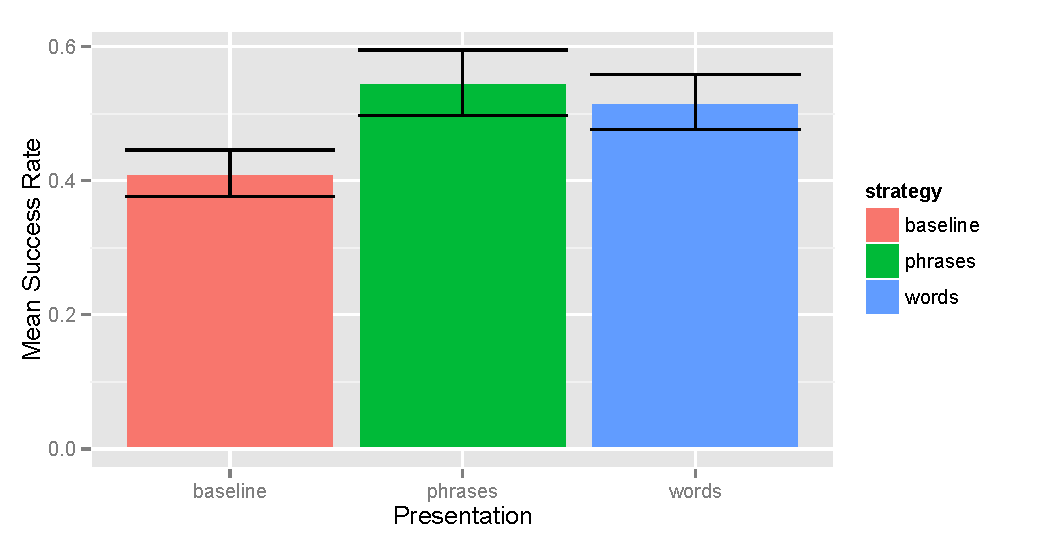
\includegraphics[width=1.0\columnwidth]{fig/overall-success-rates}
\caption{
	\label{fig:overall-success-rates} Average recognition success rates for the three different presentations.
}
\end{figure}
Our results (Figure \ref{fig:overall-success-rates}) confirm that examples improve the recognizability of grammatical relations. Participants in the \strong{baseline} condition were significantly worse at identifying the relations than participants in conditions that showed examples (\strong{phrases} and \strong{words}).  The average success rate (where success means that the participant correctly identified the relation) in the \strong{baseline} condition was $41\%$, which is significantly\footnote{Using the Wilcoxson signed-rank test, an alternative to the standard T-test that does not assume samples are normally distributed.} less accurate than in the two example-showing conditions: \strong{words}: $52\%, (p = 0.00019)$, and \strong{phrases} condition : $55\%, (p = 0.00013)$.

The difference between the two types of examples,  \strong{phrases} and \strong{words},  was not significant overall, but the data revealed an interesting fact when they were compared across the different types  of relations (Figure \ref{fig:results-by-relation-type}). In all cases, the baseline performs worse that an example-showing presentation. However, the three different categories of relations behaved very differently with respect to whether phrases or words was better.

\begin{figure}
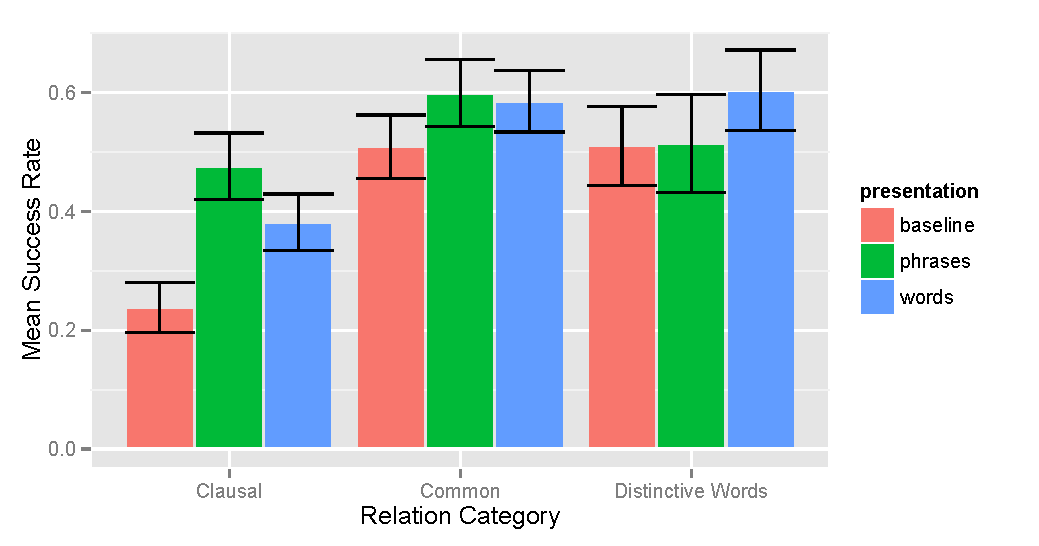
\includegraphics[width=1.0\columnwidth]{fig/by-relation-type}
\caption{
	\label{fig:results-by-relation-type} Average recognition success rates for the three categories of relations, by presentation.
}
\end{figure}


For the clausal relations, which operate over longer distances in sentences, the data confirmed what one might intuitively expect. Phrases, which show the usage context, significantly improved recognizability compared to the list of words or the baseline labels. The average success rate is 48\% for \strong{phrases}, which is significantly more than \strong{words}: 38\%, (p = 0.017), or \strong{baseline}: 24\%, ($p= 1.9 \times 10^9$).

For the common relations, there was no real difference between \strong{phrases} and \strong{words}, although they were both still significantly better than the baseline (words: $p=0.033$, phrases: $p=0.027$).

The distinctive-word relations were the opposite. These relations seem to be most recognizable when lists of words are shown instead of phrases. The average success rate in the \strong{words} case was 60\%, whereas the \strong{baseline} and \strong{phrases} cases were both 51\%. The differences, however, were suggestive, but not quite significant (words vs. baseline: $p= 0.071$, words vs. phrases: $p= 0.11$). However, we may not have had enough power to detect that difference: the other categories of relations had 4 or more relations each, but in the distinctive-words case, there were only 2 relations (adverb-modifier and noun-compound), giving us only half the data.

We therefore decided to do a follow-up experiment to gather more data.

\bibliographystyle{acm-sigchi}
\bibliography{papers}

\end{document}


\section{Experiment 2}
We hypothesized that words were more helpful when the relations involved distinctive or closed-class words: adverbs are distinctive because they usually end in `ly' -- thoughtfully, helpfully, quickly, etc. Closed-class words include determiners (a, the, that, etc.), pronouns and prepositions.  Our follow-up hypothesis was:

\begin{quote}
	H2. If distinctive or closed-class words enter into a grammatical relation, then showing a list of matching words makes it easier to recognize the relation. In other cases, a list of example phrases is more helpful.
\end{quote}

We conducted a follow-up study to verify this hypothesis. This study was had the same design as the first study: a series of identification tasks in which there was a query word and a relationship. The participants  were shown a list of sentences containing that relationship between the query word and other words, their task was to identify which relationship it was, from a list of 4 choices. Except this time, instead of presenting all the choices in the same way (as a list of matching words, or a list of matching phrases) we presented each choice in the way we thought would be most useful according to our hypothesis. If the hypothesis was true, participants in this `optimal presentation' condition would outperform participants who had all the options presented in the same way.

The results from this follow-up experiment  confirmed our hypothesis.
